%!TEX root = ../main.tex
%
%
\begin{figure}[t!]
\centering
\footnotesize
\begin{tabular}{@{}c@{\;}c@{\;}c@{\;}c@{}}
& Samples & Power spectrum & Radial mean \\
%
%=====================
%
\rotatebox{90}{\qquad\quad Random} & 
\begin{tikzpicture}
  \node[anchor=south west,inner sep=0] (image) at (0,0)
  {
    \pdfliteral{ 1 w}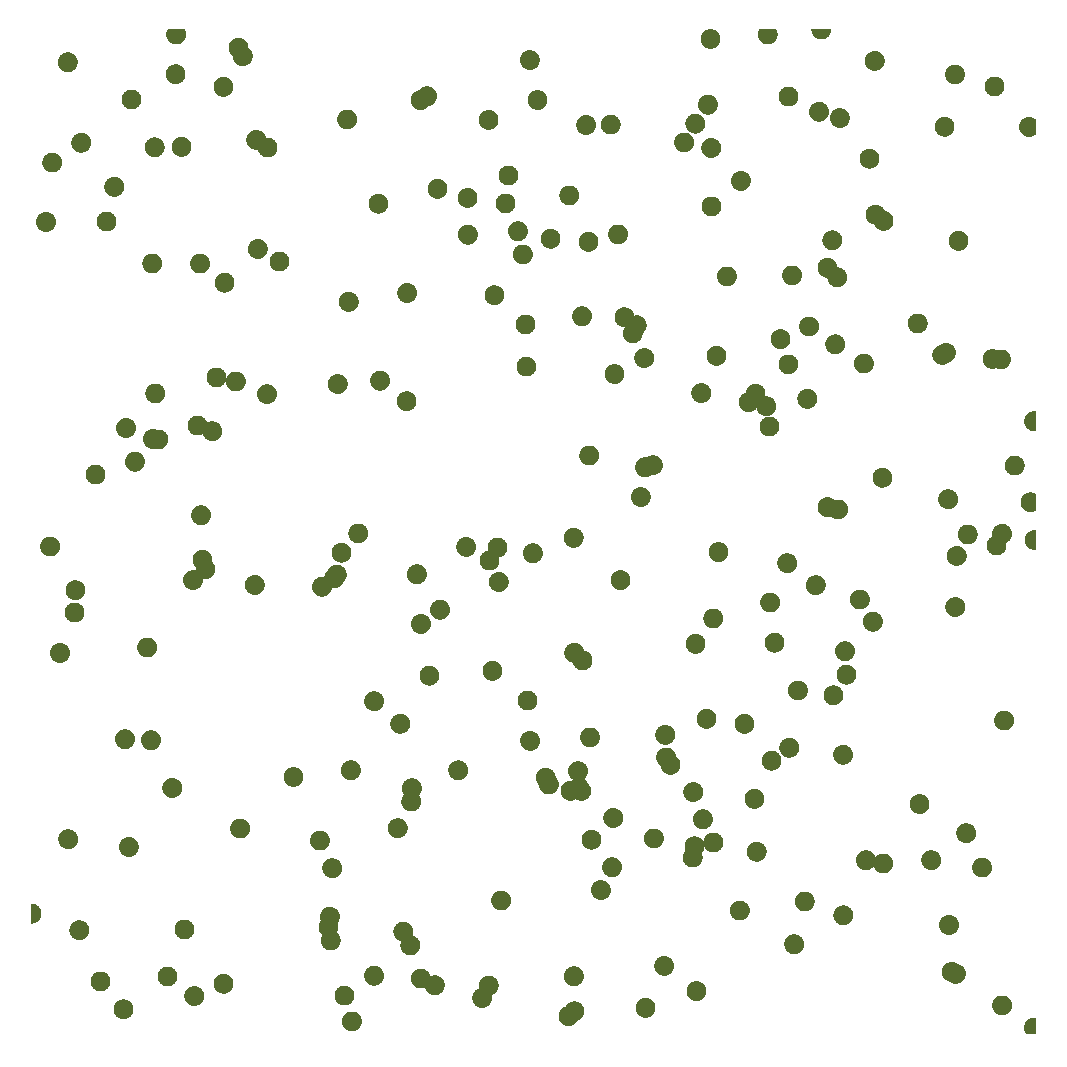
\includegraphics[width=0.2\columnwidth,page=1]{pointset/points-random-n256.pdf}
  };

  \begin{scope}[x={(image.south east)},y={(image.north west)}]
  \draw[black,thick] (0,0) rectangle (1,1);
  \end{scope}
\end{tikzpicture} 
&
\begin{tikzpicture}
  \node[anchor=south west,inner sep=0] (image) at (0,0)
  {
    \pdfliteral{ 1 w}
\includegraphics[width=0.2\columnwidth,page=1]{power-spectra/powerspectrum-random-n4096.png}
  };

  \begin{scope}[x={(image.south east)},y={(image.north west)}]
  \draw[black,thick] (0,0) rectangle (1,1);
  \end{scope}
\end{tikzpicture}
&
\begin{tikzpicture}
  \node[anchor=south west,inner sep=0] (image) at (0,0)
  {
    \pdfliteral{ 1 w}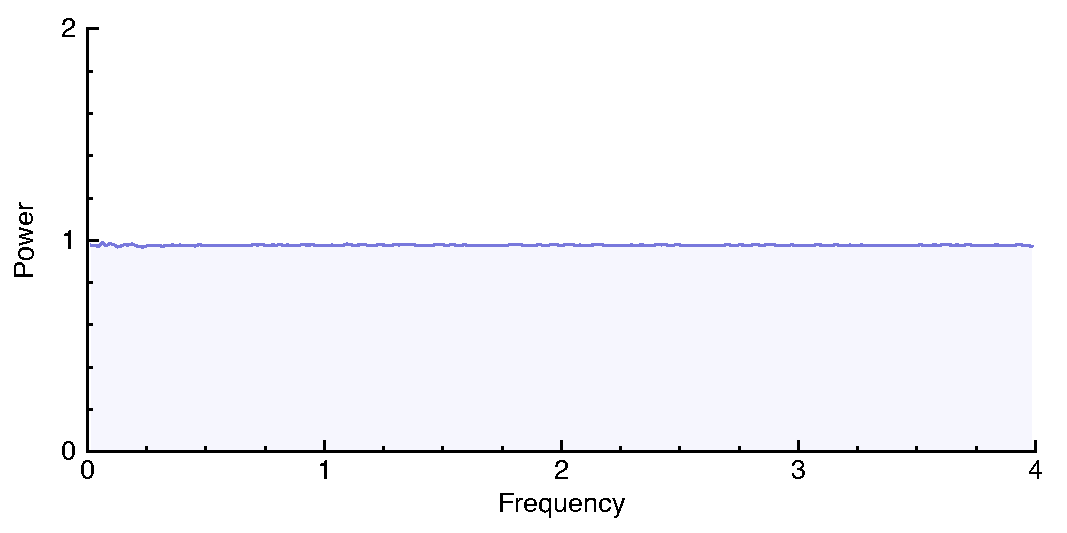
\includegraphics[width=0.4\columnwidth,page=1]{power-spectra/radial-mean-random-n4096.pdf}
  };

  \begin{scope}[x={(image.south east)},y={(image.north west)}]
  \draw[black,thick] (0,0) rectangle (1,1);
  \end{scope}
\end{tikzpicture}\\
%
%=====================
%
\rotatebox{90}{\qquad\quad Jitter} & 
\begin{tikzpicture}
  \node[anchor=south west,inner sep=0] (image) at (0,0)
  {
    \pdfliteral{ 1 w}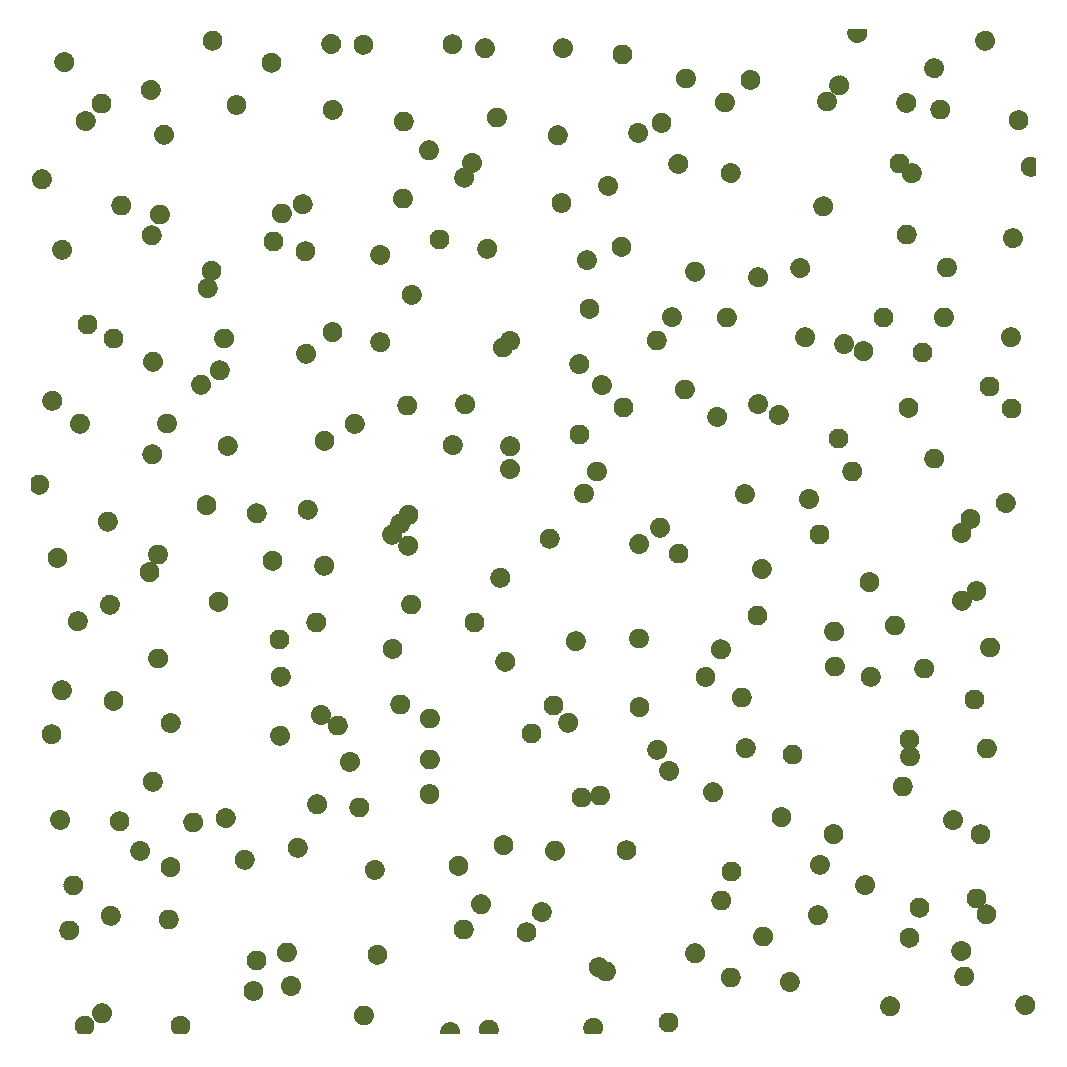
\includegraphics[width=0.2\columnwidth,page=1]{pointset/points-jitter-n256.pdf}
  };

  \begin{scope}[x={(image.south east)},y={(image.north west)}]
  \draw[black,thick] (0,0) rectangle (1,1);
  \end{scope}
\end{tikzpicture} 
&
\begin{tikzpicture}
  \node[anchor=south west,inner sep=0] (image) at (0,0)
  {
    \pdfliteral{ 1 w}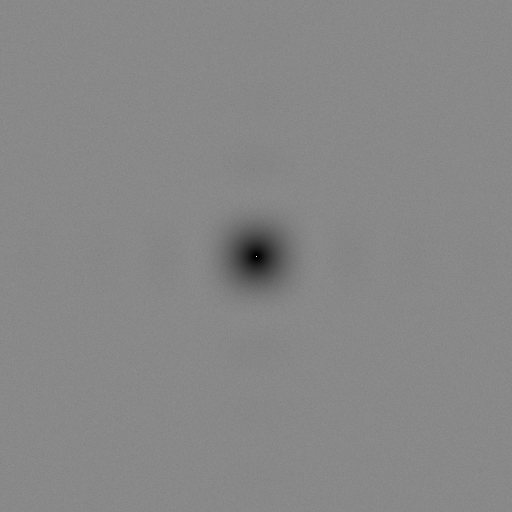
\includegraphics[width=0.2\columnwidth,page=1]{power-spectra/powerspectrum-jitter-n4096.png}
};

  \begin{scope}[x={(image.south east)},y={(image.north west)}]
  \draw[black,thick] (0,0) rectangle (1,1);
  \end{scope}
\end{tikzpicture}
&
\begin{tikzpicture}
  \node[anchor=south west,inner sep=0] (image) at (0,0)
  {
    \pdfliteral{ 1 w}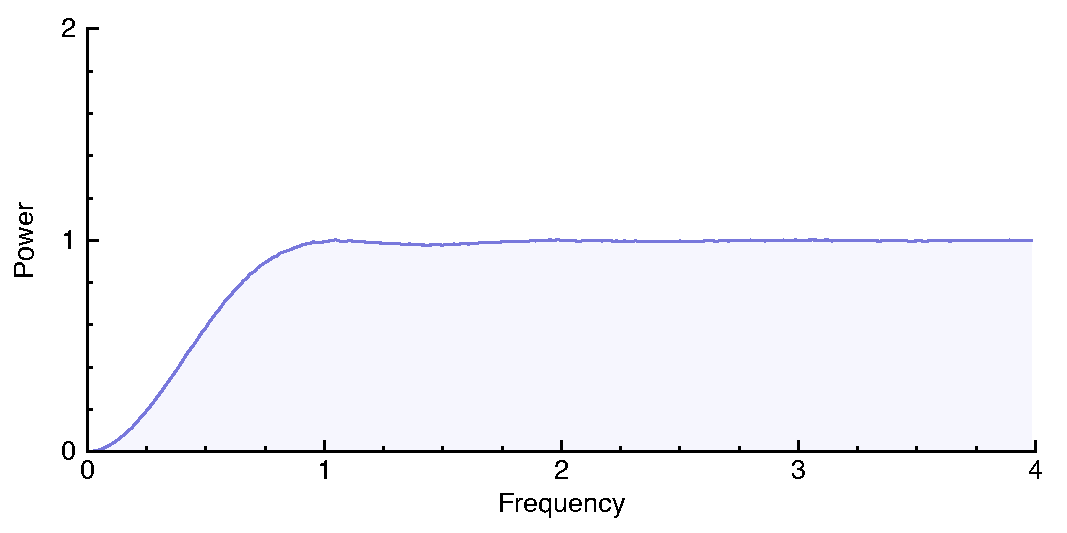
\includegraphics[width=0.4\columnwidth,page=1]{power-spectra/radial-mean-jitter-n4096.pdf}
  };

  \begin{scope}[x={(image.south east)},y={(image.north west)}]
  \draw[black,thick] (0,0) rectangle (1,1);
  \end{scope}
\end{tikzpicture}\\
%
%=====================
%
\rotatebox{90}{\quad\quad MultiJitter} & 
\begin{tikzpicture}
  \node[anchor=south west,inner sep=0] (image) at (0,0)
  {
    \pdfliteral{ 1 w}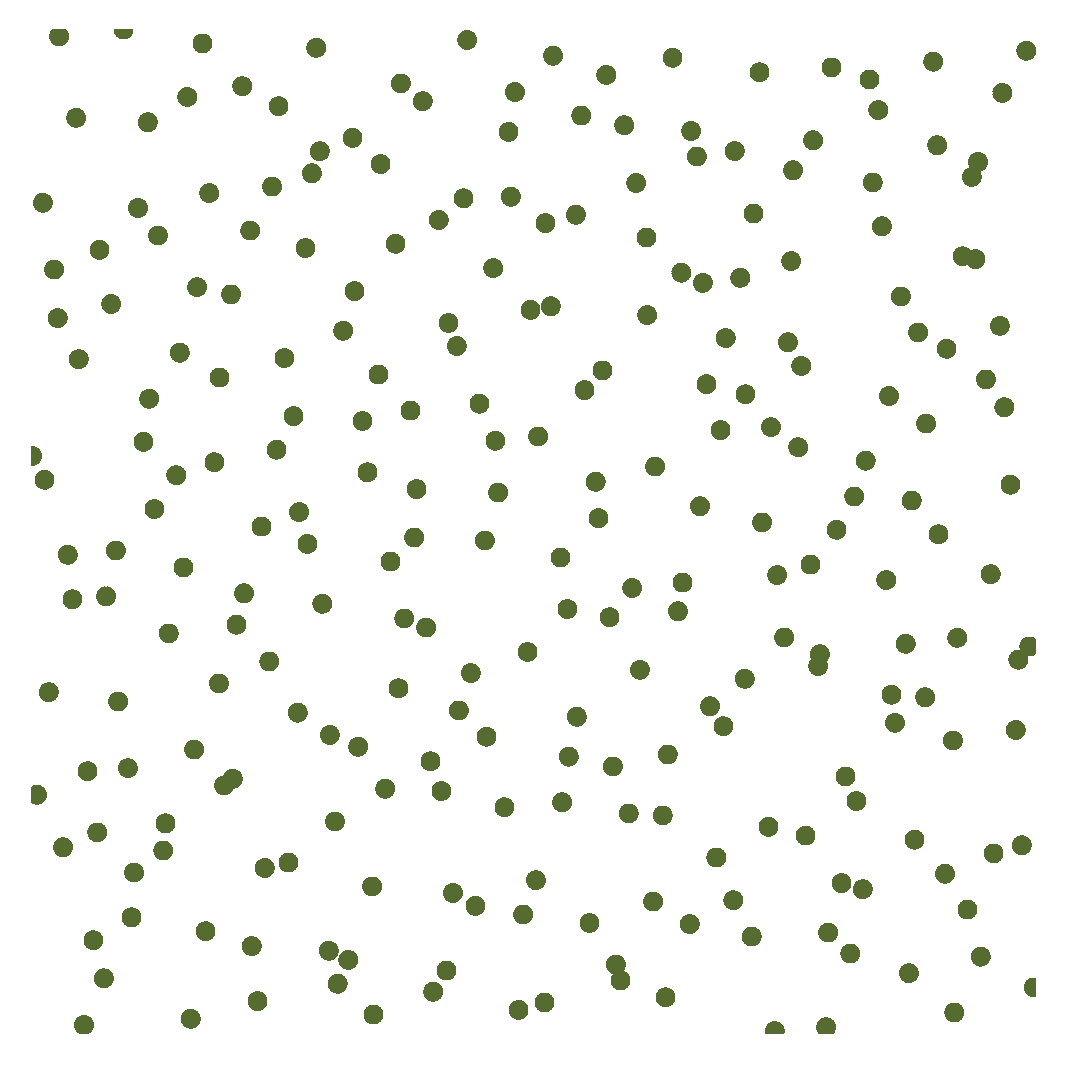
\includegraphics[width=0.2\columnwidth,page=1]{pointset/points-multijitter-n256.pdf}
  };

  \begin{scope}[x={(image.south east)},y={(image.north west)}]
  \draw[black,thick] (0,0) rectangle (1,1);
  \end{scope}
\end{tikzpicture} 
&
\begin{tikzpicture}
  \node[anchor=south west,inner sep=0] (image) at (0,0)
  {
    \pdfliteral{ 1 w}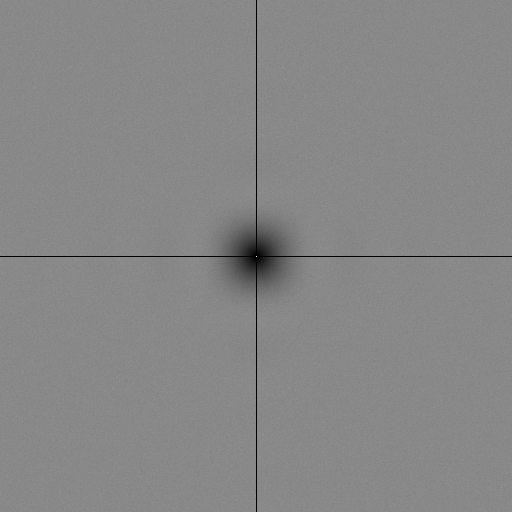
\includegraphics[width=0.2\columnwidth,page=1]{power-spectra/powerspectrum-multijitter-n4096.png}
  };

  \begin{scope}[x={(image.south east)},y={(image.north west)}]
  \draw[black,thick] (0,0) rectangle (1,1);
  \end{scope}
\end{tikzpicture}
&
\begin{tikzpicture}
  \node[anchor=south west,inner sep=0] (image) at (0,0)
  {
    \pdfliteral{ 1 w}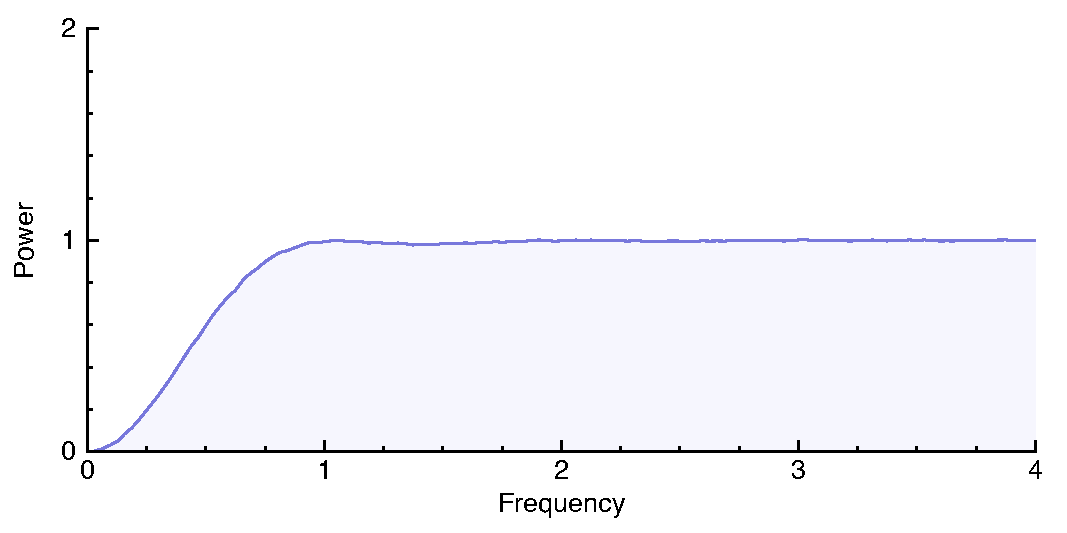
\includegraphics[width=0.4\columnwidth,page=1]{power-spectra/radial-mean-multijitter-n1024.pdf}
  };

  \begin{scope}[x={(image.south east)},y={(image.north west)}]
  \draw[black,thick] (0,0) rectangle (1,1);
  \end{scope}
\end{tikzpicture}\\
%
%=====================
%
\rotatebox{90}{\qquad Dartthrowing} & 
\begin{tikzpicture}
  \node[anchor=south west,inner sep=0] (image) at (0,0)
  {
    \pdfliteral{ 1 w}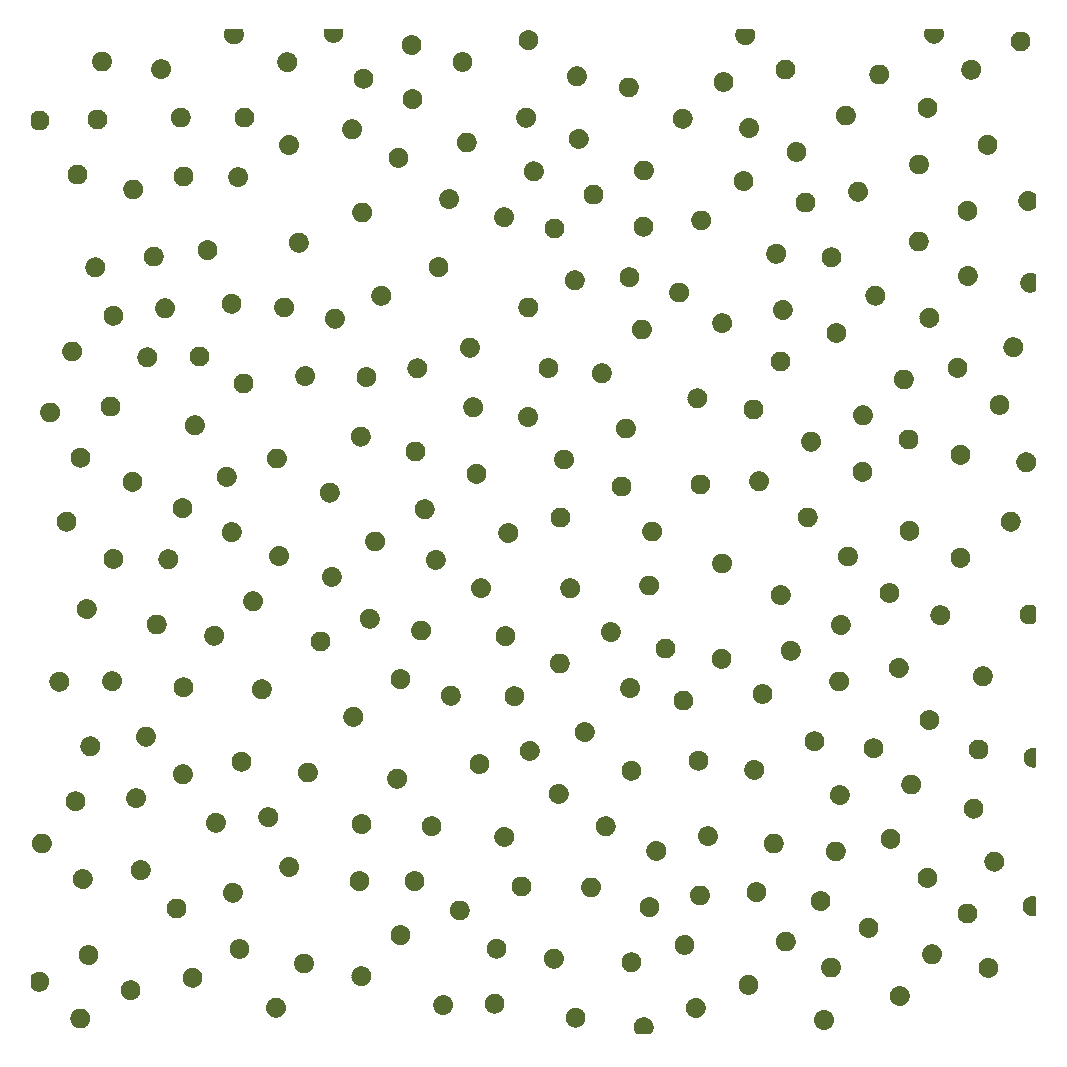
\includegraphics[width=0.2\columnwidth,page=1]{pointset/points-dartthrowing-n256.pdf}
  };

  \begin{scope}[x={(image.south east)},y={(image.north west)}]
  \draw[black,thick] (0,0) rectangle (1,1);
  \end{scope}
\end{tikzpicture} 
&
\begin{tikzpicture}
  \node[anchor=south west,inner sep=0] (image) at (0,0)
  {
    \pdfliteral{ 1 w}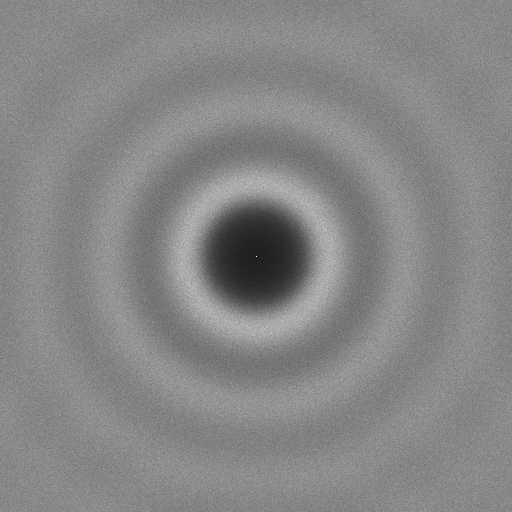
\includegraphics[width=0.2\columnwidth,page=1]{power-spectra/powerspectrum-dartthrowing-n4096.png}
  };

  \begin{scope}[x={(image.south east)},y={(image.north west)}]
  \draw[black,thick] (0,0) rectangle (1,1);
  \end{scope}
\end{tikzpicture}
&
\begin{tikzpicture}
  \node[anchor=south west,inner sep=0] (image) at (0,0)
  {
    \pdfliteral{ 1 w}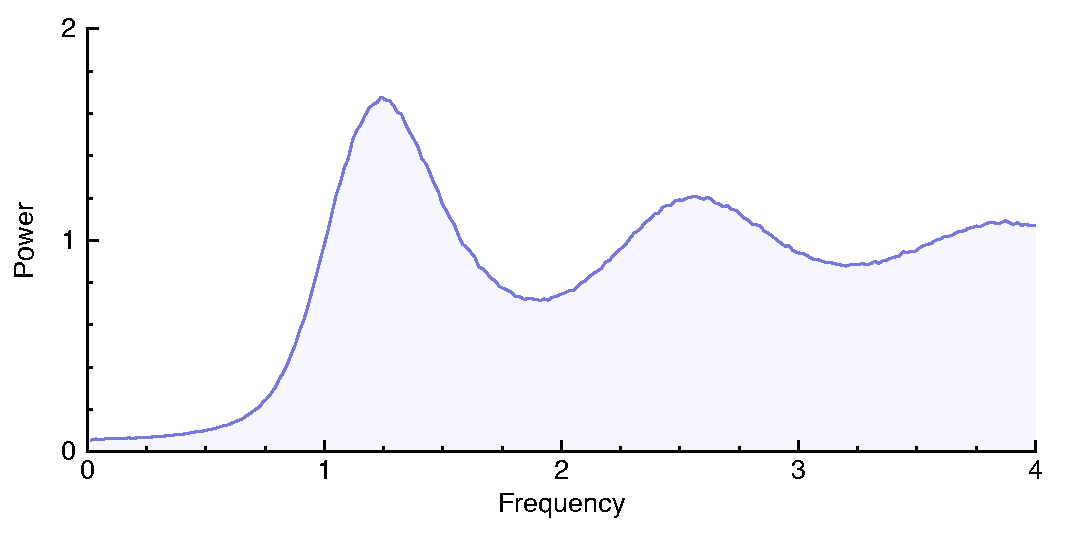
\includegraphics[width=0.4\columnwidth,page=1]{power-spectra/radial-mean-dartthrowing-n4096.pdf}
  };

  \begin{scope}[x={(image.south east)},y={(image.north west)}]
  \draw[black,thick] (0,0) rectangle (1,1);
  \end{scope}
\end{tikzpicture}\\
%
%==================
%
\rotatebox{90}{\qquad\quad Halton} & 
\begin{tikzpicture}
  \node[anchor=south west,inner sep=0] (image) at (0,0)
  {
    \pdfliteral{ 1 w}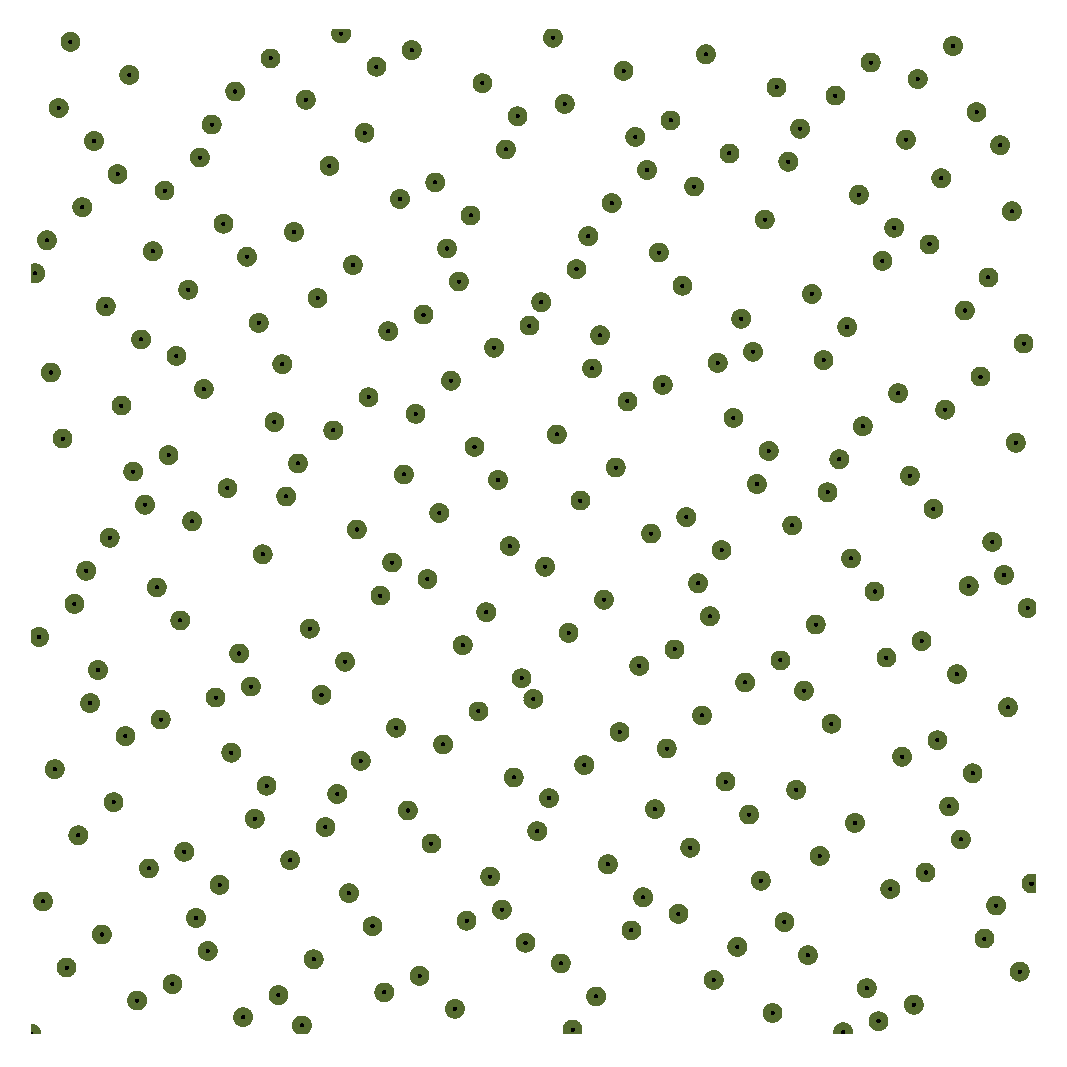
\includegraphics[width=0.2\columnwidth,page=1]{pointset/points-halton-n256.pdf}
  };

  \begin{scope}[x={(image.south east)},y={(image.north west)}]
  \draw[black,thick] (0,0) rectangle (1,1);
  \end{scope}
\end{tikzpicture} 
&
\begin{tikzpicture}
  \node[anchor=south west,inner sep=0] (image) at (0,0)
  {
    \pdfliteral{ 1 w}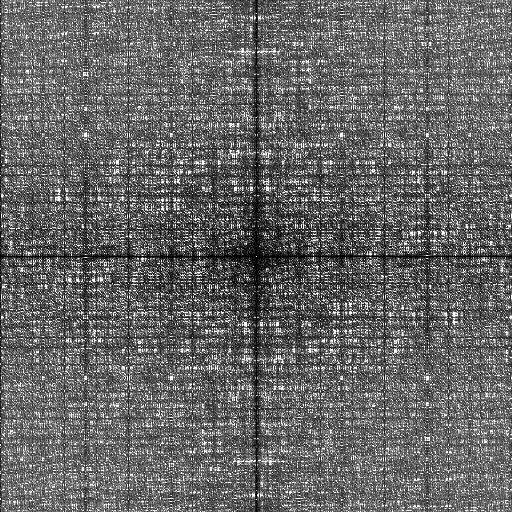
\includegraphics[width=0.2\columnwidth,page=1]{power-spectra/powerspectrum-halton-n4096.png}
  };

  \begin{scope}[x={(image.south east)},y={(image.north west)}]
  \draw[black,thick] (0,0) rectangle (1,1);
  \end{scope}
\end{tikzpicture}
&
\begin{tikzpicture}
  \node[anchor=south west,inner sep=0] (image) at (0,0)
  {
    \pdfliteral{ 1 w}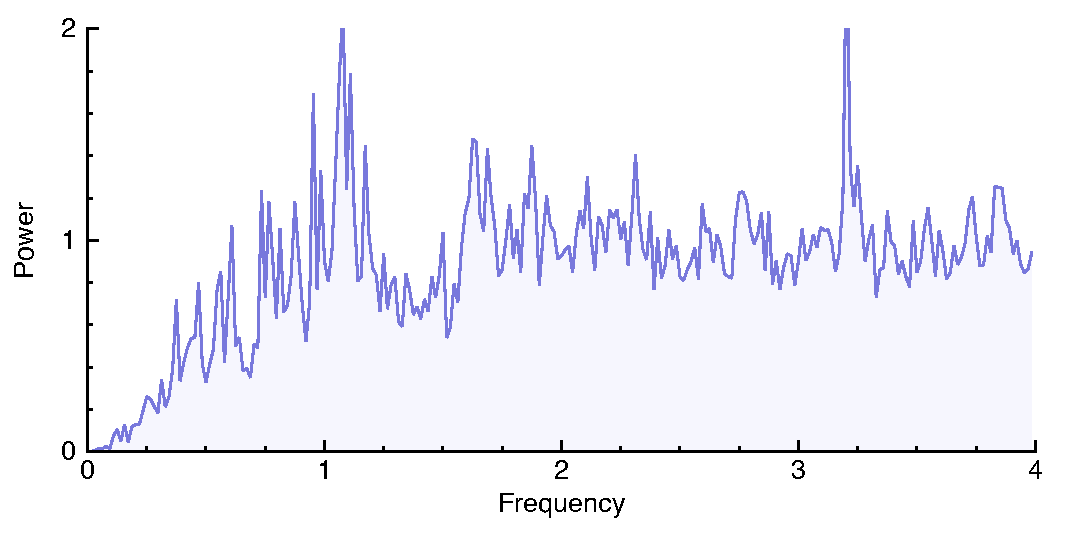
\includegraphics[width=0.4\columnwidth,page=1]{power-spectra/radial-mean-halton-n4096.pdf}
  };

  \begin{scope}[x={(image.south east)},y={(image.north west)}]
  \draw[black,thick] (0,0) rectangle (1,1);
  \end{scope}
\end{tikzpicture}\\
%
%==============
%
\rotatebox{90}{\qquad Hammerslay} & 
\begin{tikzpicture}
  \node[anchor=south west,inner sep=0] (image) at (0,0)
  {
    \pdfliteral{ 1 w}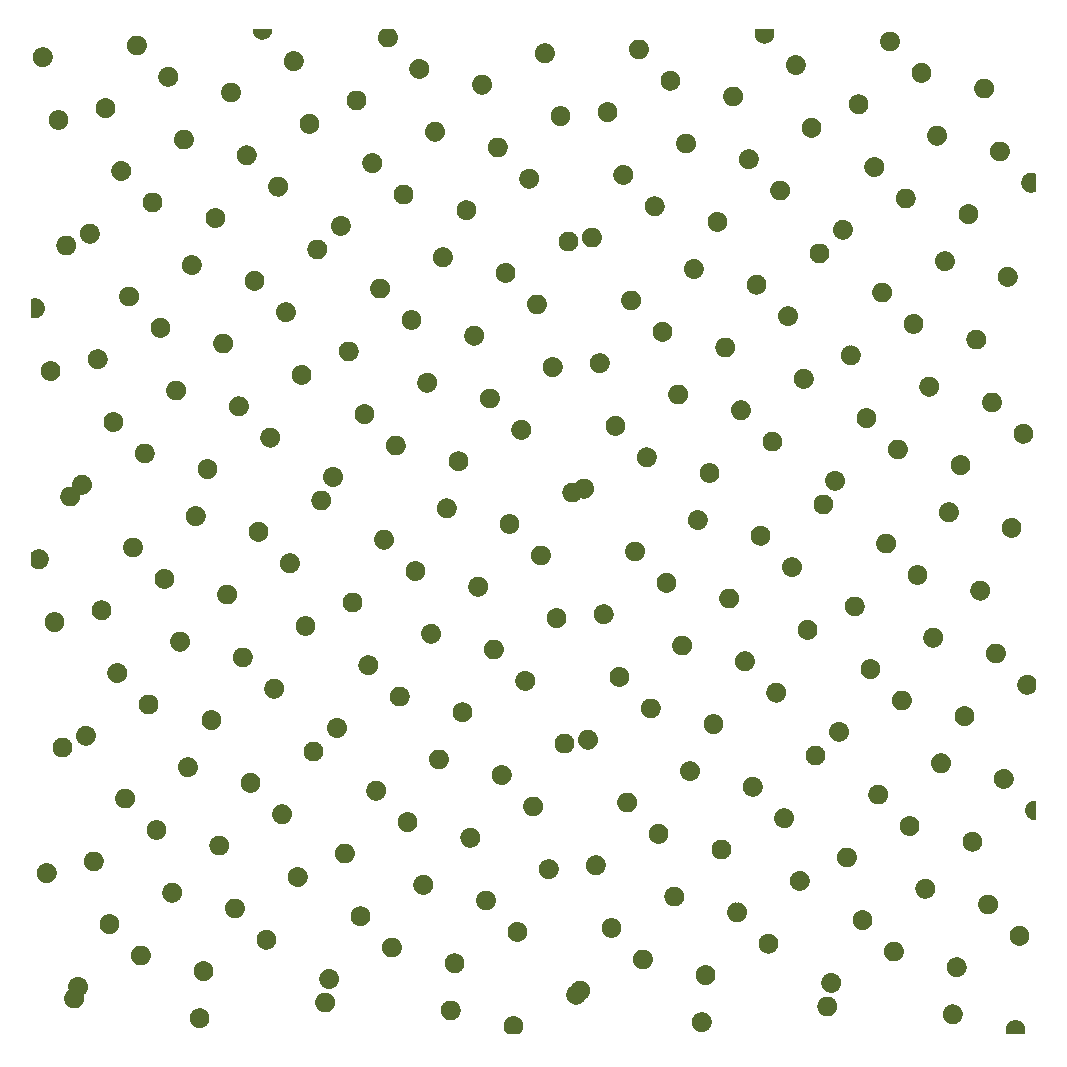
\includegraphics[width=0.2\columnwidth,page=1]{pointset/points-hammerslay-n256.pdf}
  };

  \begin{scope}[x={(image.south east)},y={(image.north west)}]
  \draw[black,thick] (0,0) rectangle (1,1);
  \end{scope}
\end{tikzpicture} 
&
\begin{tikzpicture}
  \node[anchor=south west,inner sep=0] (image) at (0,0)
  {
    \pdfliteral{ 1 w}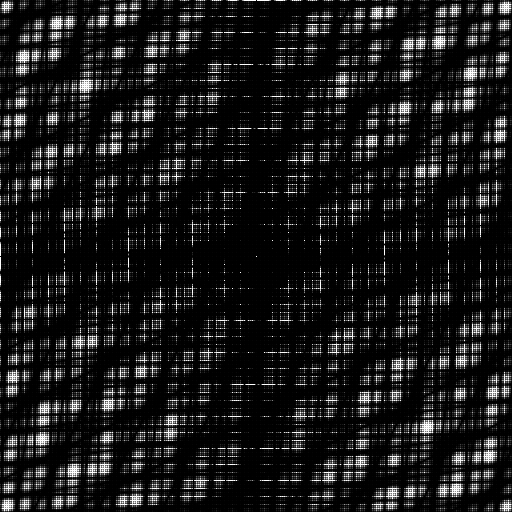
\includegraphics[width=0.2\columnwidth,page=1]{power-spectra/powerspectrum-hammerslay-n4096.png}
  };

  \begin{scope}[x={(image.south east)},y={(image.north west)}]
  \draw[black,thick] (0,0) rectangle (1,1);
  \end{scope}
\end{tikzpicture}
&
\begin{tikzpicture}
  \node[anchor=south west,inner sep=0] (image) at (0,0)
  {
    \pdfliteral{ 1 w}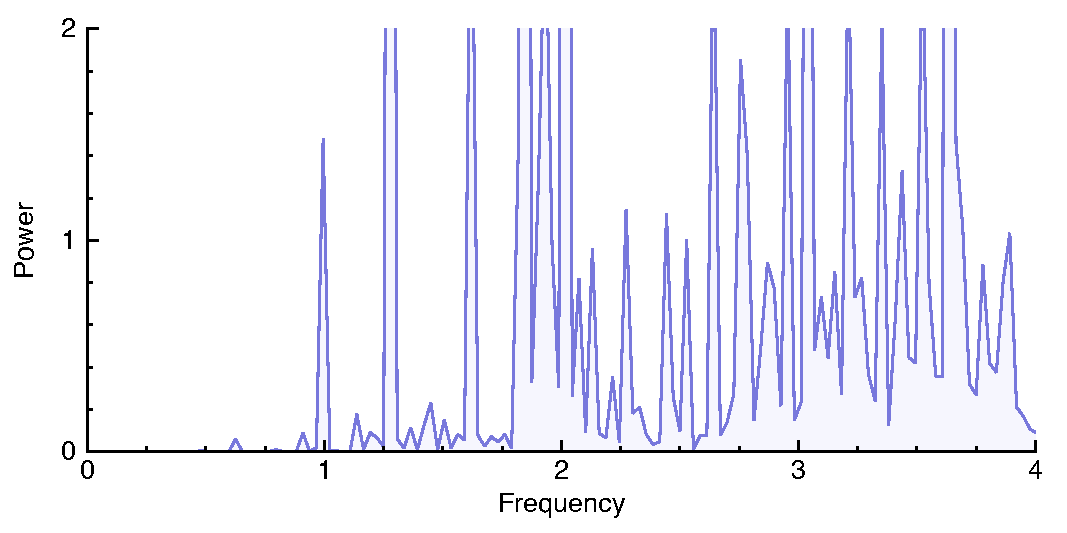
\includegraphics[width=0.4\columnwidth,page=1]{power-spectra/radial-mean-hammerslay-n4096.pdf}
  };

  \begin{scope}[x={(image.south east)},y={(image.north west)}]
  \draw[black,thick] (0,0) rectangle (1,1);
  \end{scope}
\end{tikzpicture}\\
%
%==============
%
\rotatebox{90}{\qquad\quad Regular} & 
\begin{tikzpicture}
  \node[anchor=south west,inner sep=0] (image) at (0,0)
  {
    \pdfliteral{ 1 w}
\includegraphics[width=0.2\columnwidth,page=1]{pointset/points-regular-n256.pdf}
  };

  \begin{scope}[x={(image.south east)},y={(image.north west)}]
  \draw[black,thick] (0,0) rectangle (1,1);
  \end{scope}
\end{tikzpicture} 
&
\begin{tikzpicture}
  \node[anchor=south west,inner sep=0] (image) at (0,0)
  {
    \pdfliteral{ 1 w}
\includegraphics[width=0.2\columnwidth,page=1]{power-spectra/powerspectrum-regular-n4096-cropped.png}
  };

  \begin{scope}[x={(image.south east)},y={(image.north west)}]
  \draw[black,thick] (0,0) rectangle (1,1);
  \end{scope}
\end{tikzpicture}
&
\begin{tikzpicture}
  \node[anchor=south west,inner sep=0] (image) at (0,0)
  {
    \pdfliteral{ 1 w}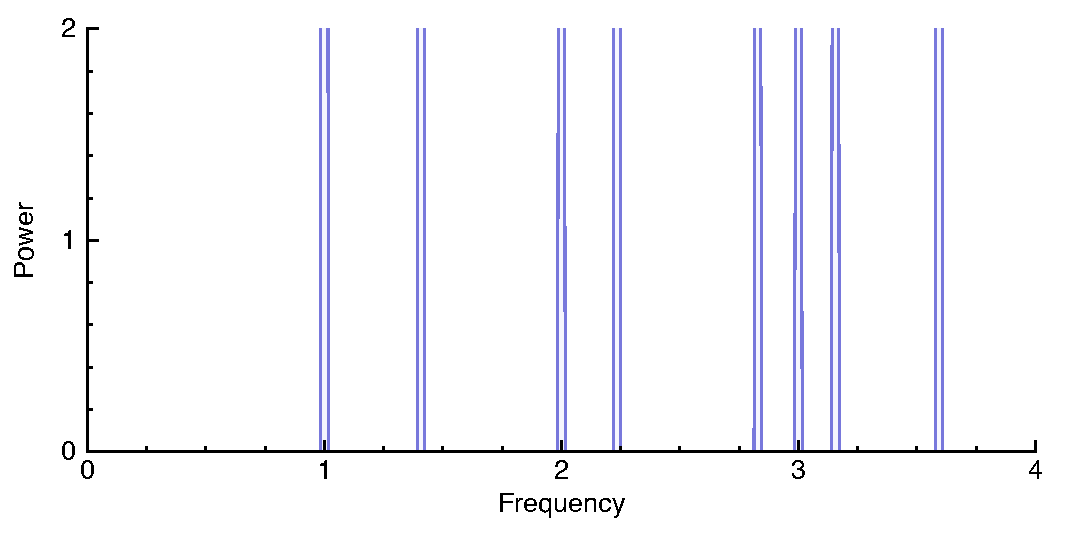
\includegraphics[width=0.4\columnwidth,page=1]{power-spectra/radial-mean-regular-n4096.pdf}
  };

  \begin{scope}[x={(image.south east)},y={(image.north west)}]
  \draw[black,thick] (0,0) rectangle (1,1);
  \end{scope}
\end{tikzpicture}\\
\end{tabular}
%
\caption{\label{fig:points-powspec-radialmean}%
Illustration of some well known sampling patterns in 2D with the corresponding Fourier expected power spectra and the corresponding radial mean of their expected power spectra.}
\end{figure}